\documentclass[10pt,aspectratio=169]{beamer}

\usetheme{metropolis}
\usepackage{booktabs}
\usepackage{xcolor}
\usepackage{hyperref}
\usepackage{graphicx}
\usepackage{pgfpages}
\setbeameroption{show notes on second screen=right}

% ---------------------------------------------------------------------
% Yale colors (https://usebrand.yale.edu/colors)
% ---------------------------------------------------------------------
\definecolor{YaleBlue}{HTML}{00356B}
\definecolor{YaleBlueLight}{HTML}{286DC0}
\definecolor{YaleGray}{HTML}{4A4A4A}
\definecolor{YaleGrayLight}{HTML}{DDDDDD}
\definecolor{YaleAccent}{HTML}{BD5319}
\definecolor{goodgreen}{HTML}{2E8B57}

% ---------------------------------------------------------------------
% Metropolis theme overrides --- Yale Blue
% ---------------------------------------------------------------------
\setbeamercolor{normal text}{fg=black, bg=white}
\setbeamercolor{alerted text}{fg=YaleAccent}
\setbeamercolor{example text}{fg=YaleBlue}

\setbeamercolor{frametitle}{bg=YaleBlue, fg=white}
\setbeamercolor{title separator}{fg=YaleBlueLight}
\setbeamercolor{progress bar}{fg=YaleBlueLight, bg=YaleGrayLight}
\setbeamercolor{progress bar in section page}{fg=YaleBlueLight, bg=YaleGrayLight}

\setbeamercolor{section title}{fg=YaleBlue}
\setbeamercolor{subsection title}{fg=YaleBlueLight}
\setbeamercolor{standout}{bg=YaleBlue, fg=white}

\setbeamercolor{block title}{bg=YaleBlue, fg=white}
\setbeamercolor{block body}{bg=YaleGrayLight!30, fg=black}
\setbeamercolor{block title alerted}{bg=YaleAccent, fg=white}
\setbeamercolor{block body alerted}{bg=YaleGrayLight!30, fg=black}

\setbeamercolor{itemize item}{fg=YaleBlue}
\setbeamercolor{itemize subitem}{fg=YaleBlueLight}
\setbeamercolor{enumerate item}{fg=YaleBlue}

% ---------------------------------------------------------------------
% Meta
% ---------------------------------------------------------------------
\title{DJNW Metadata Audit}
\subtitle{How reliable is Dow Jones's article tagging?}
% \author{James Zhang}
% \institute{Yale University}
\date{\today}

\begin{document}

\maketitle

\begin{frame}{Outline}
  \tableofcontents
\end{frame}

% ===================================================================
\section{Motivation: DJNW metadata is unreliable}

\begin{frame}{Case study: crude oil tags in DJNW}
  \scriptsize
  Dow Jones tags each article with metadata codes. We investigated how well
  these tags identify crude-oil-relevant articles across the full 1979--2025
  archive (31.7M articles, 555 months).

  \smallskip
  Scanning all five taxonomy CSVs, we identified \textbf{16 content codes}
  plus \textbf{3 oil/energy wire codes} that could identify crude-oil articles:

  \smallskip
  \begin{tabular}{@{}llll@{}}
    \toprule
    \textbf{Code} & \textbf{Description} & \textbf{Code} & \textbf{Description} \\
    \midrule
    \multicolumn{4}{@{}l@{}}{\textit{Content codes (what the article is about)}} \\
    \texttt{N/PET}  & Crude Oil \& Petroleum Products        & \texttt{I/OIL}  & Major Oil \& Gas \\
    \texttt{N/CMKT} & Crude Spot Market Commentary           & \texttt{I/OIS}  & Oil Extraction \\
    \texttt{N/PRD}  & Oil \& Natural Gas Production          & \texttt{I/FSL}  & Fossil Fuels \\
    \texttt{N/OPC}  & OPEC                                   & \texttt{M/ENE}  & Energy market \\
    \texttt{N/REF}  & Refinery Outages                       & \texttt{S/OIL}  & Oil \\
    \texttt{N/RMKT} & Refined Products Spot Market Commentary & \texttt{S/API}  & API Weekly Statistics \\
    \texttt{N/RPRI} & Refined Products Spot Market Prices    & \texttt{S/DOE}  & DOE Weekly Data \\
    \texttt{N/ENY}  & Energy                                 & \texttt{N/EGY}  & Energy Commentary \\
    \midrule
    \multicolumn{4}{@{}l@{}}{\textit{Wire codes (which DJ service carried the article)}} \\
    \texttt{N/IPR}  & International Petroleum Report         & \texttt{N/DOI}  & DJ Oil \& Gas Service \\
    \texttt{N/NRG}  & Dow Jones Energy Service               & & \\
    \bottomrule
  \end{tabular}

  \smallskip
  Note: ``WTI'' and ``Brent'' are \emph{not} DJNW codes --- they are words
  in headlines. DJNW uses \texttt{N/PET} for both.
\end{frame}

\begin{frame}{Content codes: absolute usage over time}
  \centering
  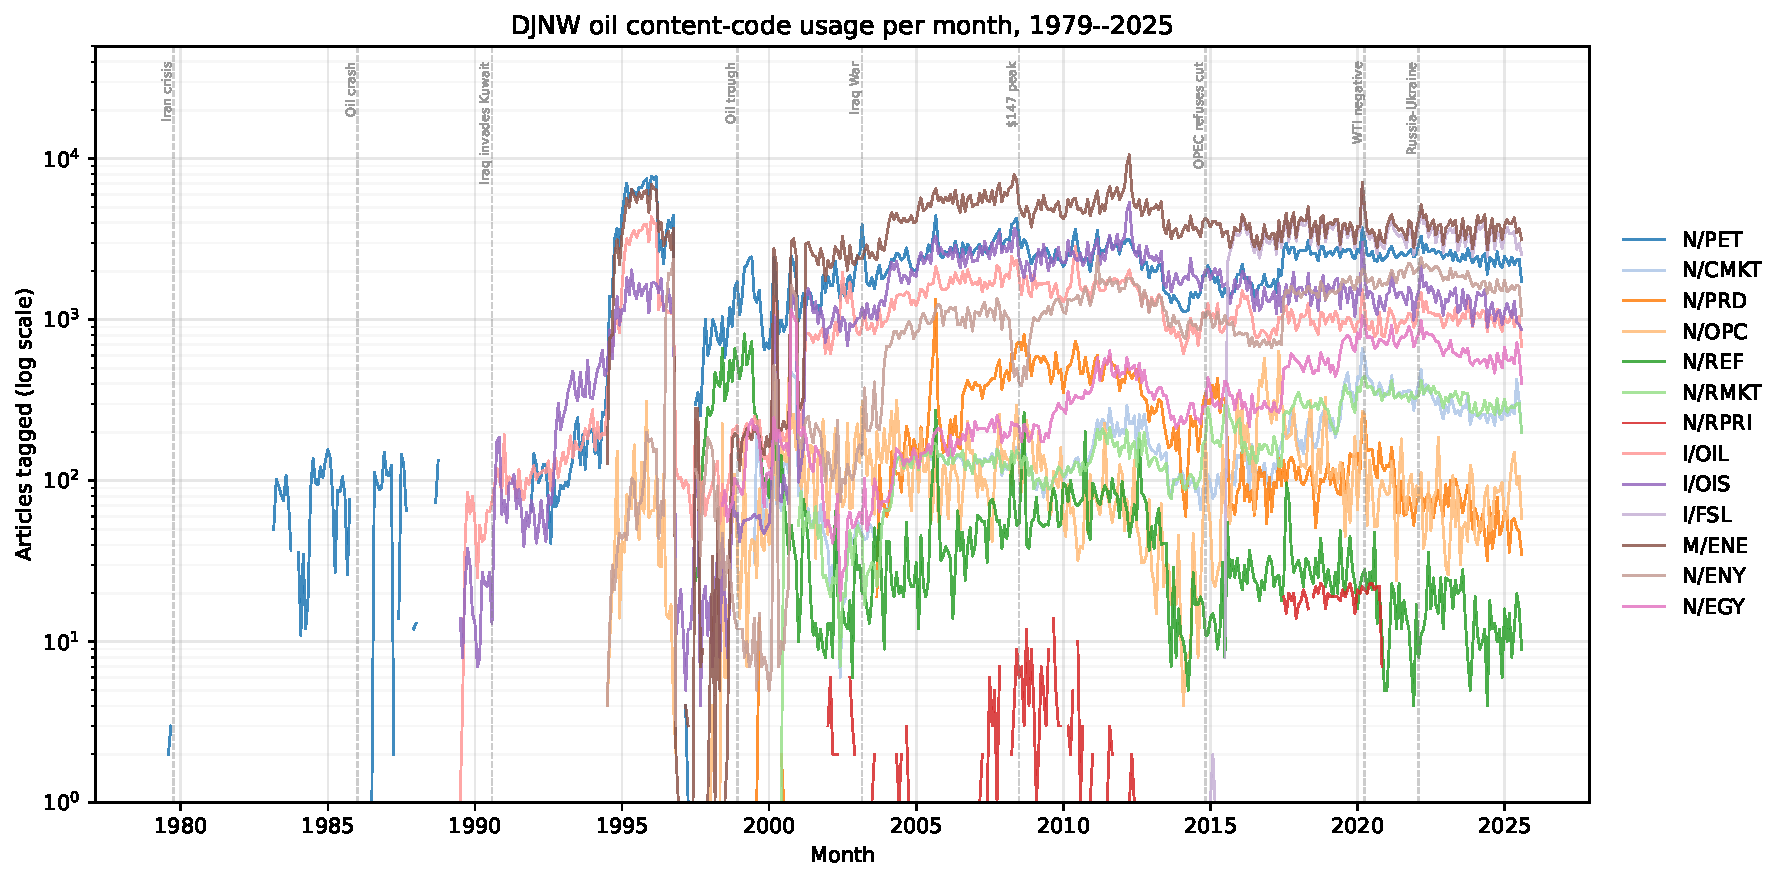
\includegraphics[width=0.9\textwidth]{crude_tags_absolute.pdf}

  \scriptsize
  Log scale, monthly. Most content codes do not appear until the mid-1990s.
\end{frame}

\begin{frame}{Wire codes: absolute usage over time}
  \centering
  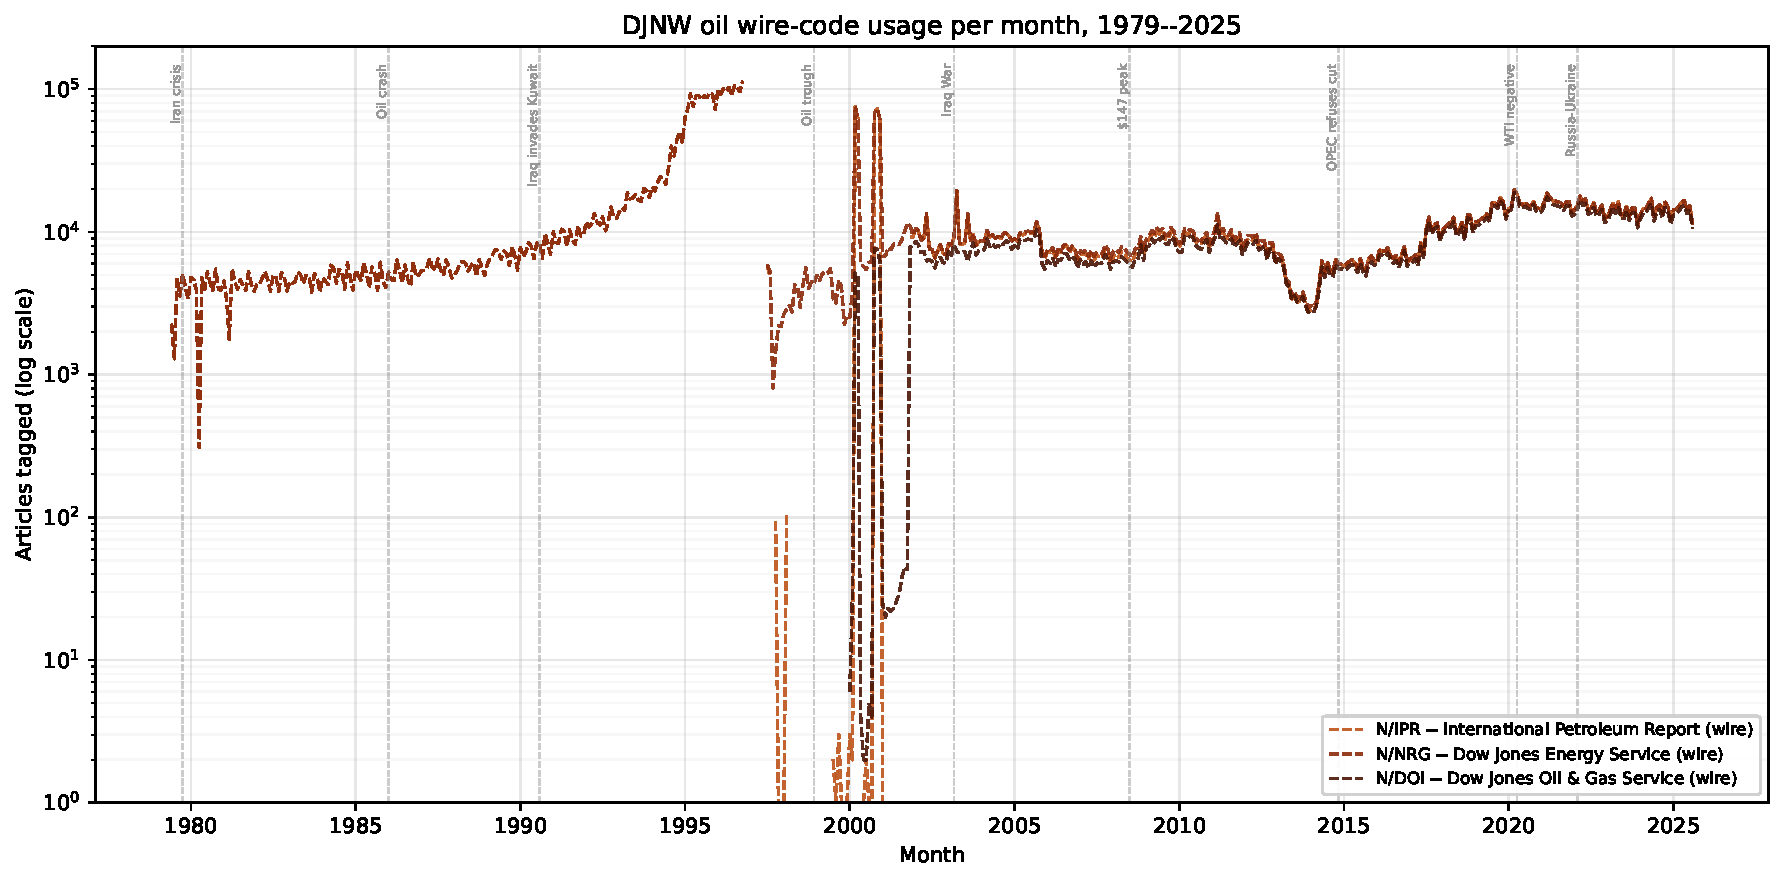
\includegraphics[width=0.9\textwidth]{crude_tags_absolute_wire.pdf}

  \scriptsize
  Log scale, monthly. Wire codes saturate at $\sim$100k articles/month from
  1979 onwards (they were stamped on everything), then drop sharply at
  Nov 1996 and stabilize at a lower volume.
\end{frame}

\begin{frame}{Content codes: share of articles carrying each tag}
  \centering
  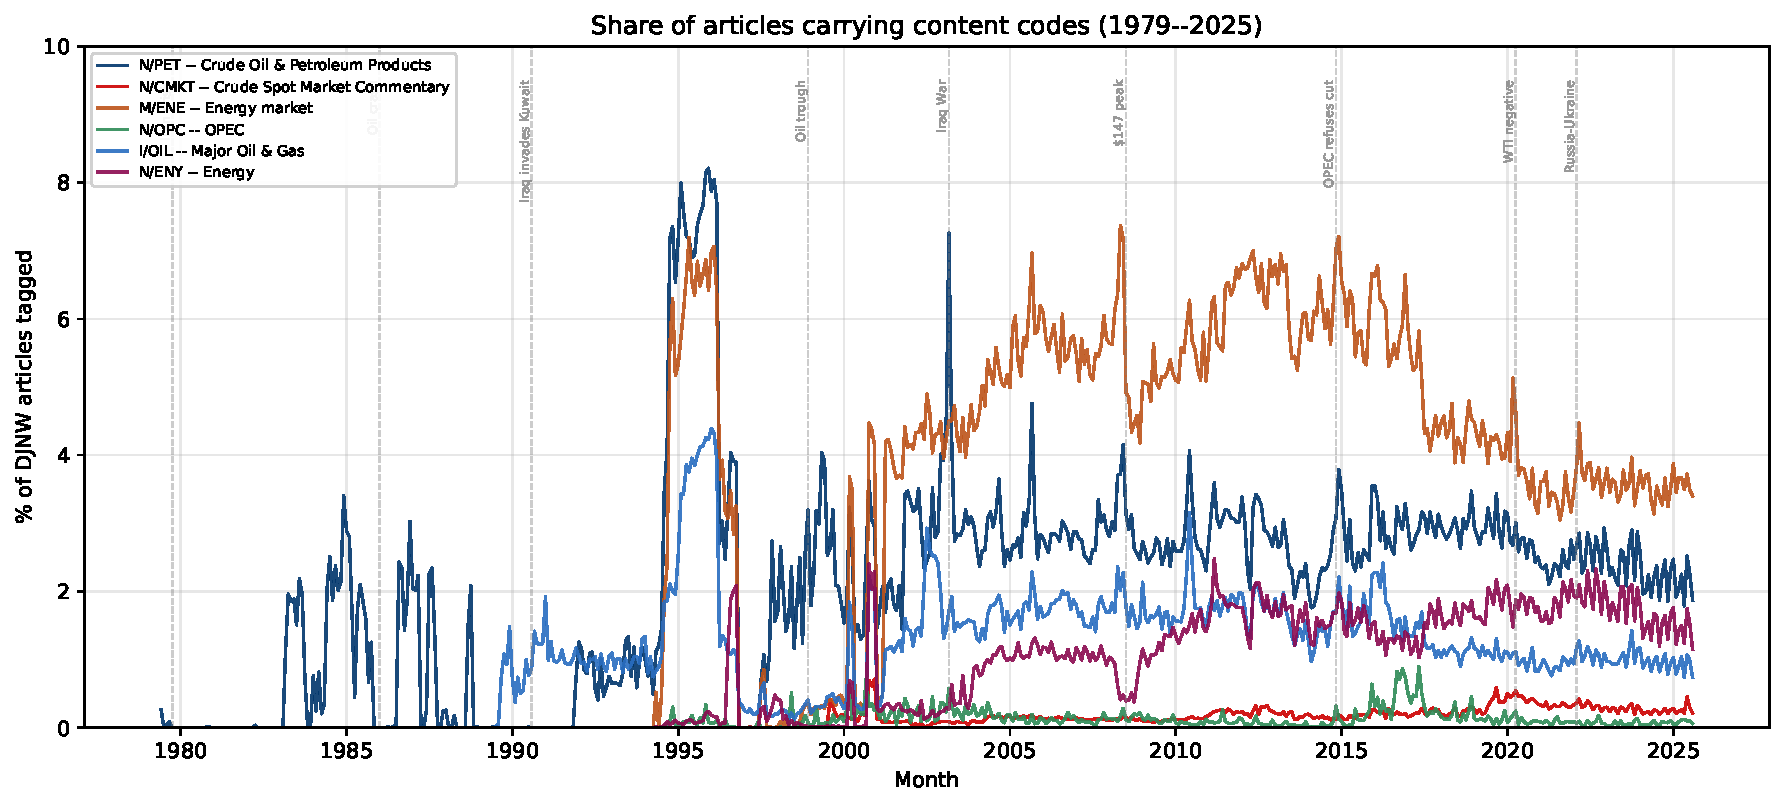
\includegraphics[width=0.9\textwidth]{crude_tags_percentage.pdf}

  \scriptsize
  Baseline is sparse --- no code exceeds $\sim$8\% even at peaks.
\end{frame}

\begin{frame}{Wire codes: share of articles carrying each tag}
  \centering
  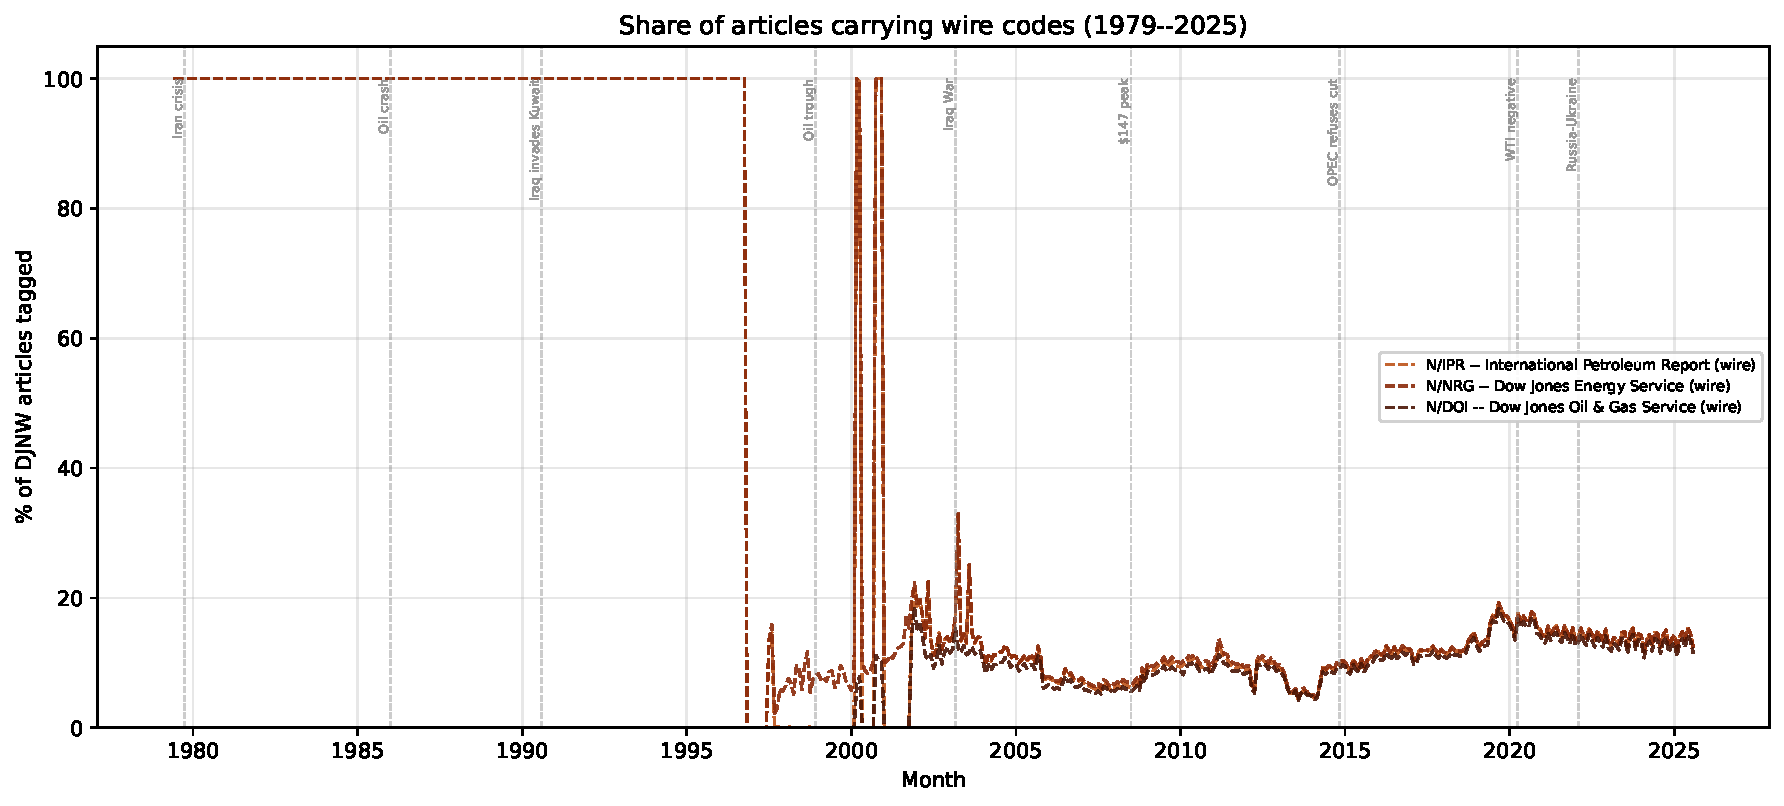
\includegraphics[width=0.9\textwidth]{crude_tags_wire_percentage.pdf}

  \scriptsize
  Wire codes: 100\% spam pre-Nov 1996, brief regressions in
  Mar/Apr/Oct--Dec 2000, then selective ($\sim$10--20\%) from 2001.
  Post-2000, \texttt{N/IPR} is a useful weak positive signal.
\end{frame}

\begin{frame}{Recall failure 1: direct oil reporting without oil tags}
  \scriptsize
  Articles where crude oil \emph{is the primary subject} yet carry
  \textbf{none} of the 19 oil codes:

  \smallskip
  \begin{itemize}
    \item \textit{``Economic Outlook 99: Saudi Arabia Hurt By Low Oil Prices''} (1998-12-14)
    \item \textit{``Saudi Oil Price Cut Dings Energy ETFs''} (2014-11-04, Barron's)
    \item \textit{``Venezuela Serves Up a Culture Shock for Visiting Saudi Oil Minister''} (2014-11-07)
    \item \textit{``Russia to Pump Up Oil Exports to Asia''} (2014-12-04)
    \item \textit{``Abu Dhabi's Mubadala Wealth Fund Swings to Loss on Low Oil Prices''} (2016-09-08)
    \item \textit{``Nymex Crude Biased Down Near-Term; \$78.08 Support''} (2014-11-03)
    \item \textit{``Exxon to Shut Down Oil Production in Russia After Ukraine Attack''} (2022-03-01)
  \end{itemize}

  \smallskip
  These are exactly the articles a macro researcher searching for OPEC, Saudi,
  or petro-state policy \emph{should} find by tag. All missed.

  \note{
    \scriptsize
    \textbf{Verification} (all in \texttt{.../rc2573/output/cleaned/v2/articles/}): \\[2pt]
    \texttt{19981214001135} in \texttt{1998-12a\_clean.jsonl} \\
    \texttt{20141104009555}, \texttt{20141107013622} in \texttt{2014-11a\_clean.jsonl} \\
    \texttt{20141204001090} in \texttt{2014-12a\_clean.jsonl} \\
    \texttt{20160908005314} in \texttt{2016-09a\_clean.jsonl} \\
    \texttt{20141103015258} in \texttt{2014-11a\_clean.jsonl} \\
    \texttt{20220301015891} in \texttt{2022-03a\_clean.jsonl} \\[2pt]
    All verified against the 19-code set (16 content + N/IPR, N/NRG, N/DOI). \\
    Full results: \texttt{results/missing\_oil\_tags\_v3.txt} (930 DIRECT cases across 20 event months).
  }
\end{frame}

\begin{frame}{Recall failure 2: cross-asset articles reacting to oil}
  \scriptsize
  Articles about FX, equities, or bonds \emph{reacting to oil} also
  frequently lack oil codes --- even though the article's thesis is
  literally ``asset $X$ moves because of oil'':

  \smallskip
  \begin{itemize}
    \item \textit{``Canadian Dollar Ends Sharply Down on Lower Oil Prices, Dovish Poloz''} (2014-11-03)
    \item \textit{``Ruble Hits New Low as Oil Prices Drop''} (2014-12-01)
    \item \textit{``NZ Shares Fall as Saudi Attack Sends Oil Price Gushing''} (2019-09-15, post-Abqaiq)
    \item \textit{``Shares in European Airlines Fall as Oil Price Jumps''} (2020-01-03, post-Soleimani)
    \item \textit{``Falling Oil Prices Help Cruise, Airline Stocks''} (2023-10-04, Israel-Gaza)
    \item \textit{``Stock Futures Fall as Oil Rises Back Above \$100''} (2022-03-01)
  \end{itemize}

  \smallskip
  \textbf{Arguably gray-zone} --- DJ might reasonably not tag these as ``oil''
  (the subject is the reacting asset). But for research on oil's
  macroeconomic effects, these are exactly the articles we'd want surfaced.

  \note{
    \scriptsize
    \textbf{Verification} (all in \texttt{.../rc2573/output/cleaned/v2/articles/}): \\[2pt]
    \texttt{20141103012721} in \texttt{2014-11a\_clean.jsonl} \\
    \texttt{20141201007859} in \texttt{2014-12a\_clean.jsonl} \\
    \texttt{20190915001150} in \texttt{2019-09b\_clean.jsonl} \\
    \texttt{20200103001619} in \texttt{2020-01a\_clean.jsonl} \\
    \texttt{20231004005536} in \texttt{2023-10a\_clean.jsonl} \\
    \texttt{20220301002641} in \texttt{2022-03a\_clean.jsonl} \\[2pt]
    Full results: \texttt{results/missing\_oil\_tags\_v3.txt} (1,591 CROSS\_ASSET cases).
  }
\end{frame}

\begin{frame}{The wire-code problem: pre-1996 spam and the 1996 transition}
  \scriptsize
  The \texttt{N/} prefix is \textbf{overloaded} --- it mixes content tags
  with wire codes (which DJ service carried the article). In 1979--1996,
  every article was stamped with $\sim$19 identical wire codes including
  \texttt{N/IPR}, \texttt{N/NRG}, \texttt{N/DOI}. Non-energy articles carrying
  \texttt{N/IPR}:

  \smallskip
  \begin{tabular}{@{}lp{9cm}@{}}
    \toprule
    \textbf{Date} & \textbf{Headline (all have \texttt{N/IPR})} \\
    \midrule
    1985-06 & \textit{``IBM Announces New Modular Processor for Finance Industry''} \\
    1990-03 & \textit{``NV Philips Year Net Rose 30\% After Gains''} \\
    1993-06 & \textit{``Richmond Fed's Broaddus: US Econ Poised For Moderate Growth''} \\
    1993-06 & \textit{``UK May Purchasing Mgrs Index Fell To 53.0\%''} \\
    \bottomrule
  \end{tabular}

  \smallskip
  In Nov 1996, \texttt{N/IPR} coverage drops from 100\% $\to$ 0.4\% in one
  month (the same step appears across \texttt{N/NRG}, \texttt{N/DOI} --- a
  tagging-system change, \textit{inferred}). Post-1996 it stabilizes at
  10--20\% and becomes a useful weak positive signal for oil content.

  \smallskip
  \textbf{In practice:} include \texttt{N/IPR}, \texttt{N/NRG}, \texttt{N/DOI}
  post-2000 as weak positive signals. Pre-Nov 1996 and Mar/Apr/Oct--Dec 2000
  are anomalous and should be masked.

  \note{
    \textbf{Verification references} (all in \texttt{.../rc2573/output/cleaned/v2/articles/}): \\[4pt]
    \texttt{1985-06\_clean.jsonl}: 4,038/4,038 articles carry the same 19 wire codes. \\
    \texttt{19850603000003} IBM \quad \texttt{19900301000002} NV Philips \\
    \texttt{19930601000002} Richmond Fed \quad \texttt{19930601000004} UK May PMI \\[4pt]
    Share of articles carrying N/IPR: 1995-12 = 100.0\%, 1996-05 = 100.0\%,
    1996-11 = 0.4\%, 1997-01 = 0.3\%, 2022-03 = 14.8\%.
  }
\end{frame}

\begin{frame}{Precision check: picking the right code}
  \scriptsize
  \textbf{Method.} To test precision, we drew two random samples of 50
  articles each from March 2022: one from the 3,315 articles tagged
  \texttt{N/PET}, one from the 492 articles tagged \texttt{N/CMKT}
  (seed 42). We read each headline and judged whether the article is
  actually about the crude oil commodity market.

  \smallskip
  \textbf{\texttt{N/PET} (``Crude Oil \& Petroleum Products'')} is the broad
  subject umbrella --- it fires on any article touching an oil company.
  The 50-article sample surfaces substantial noise:

  \smallskip
  \textit{Clearly unrelated:} ``Stellantis Battery Plant Investment'',
  ``Income Investing: Global Dividends Surge'' (Barron's),
  ``Heard on the Street: Indian Economy on the Clock'',
  ``Australian Budget\ldots{}Balancing Act''. \\
  \textit{Oil-company corporate news (not the oil market):}
  ``Warren Buffett Gets His Deal Mojo Back'',
  ``Carl Icahn Reduces Occidental Stake'',
  ``Moody's Upgrades Murphy Oil'',
  ``ConocoPhillips to Hold Earnings Call'',
  ``VP Lannie Sells 40,800 Of APA Corp'',
  ``Equinor ASA: Share buy-back'',
  ``Exxon Mobil Down Over 6\%''.

  \smallskip
  \textbf{\texttt{N/CMKT} (``Crude Spot Market Commentary'') is the right code.}
  In the 50-article sample: the entire list is crude-market commentary ---
  WTI/Brent price moves, OPEC decisions, inventory draws, SPR releases,
  Russian oil sanctions, tanker charters. \textbf{Zero} clearly-unrelated
  articles; zero corporate filings or earnings-call press releases.

  \smallskip
  \textbf{Trade-off:} \texttt{N/CMKT} is much narrower ($\sim$15\% of
  \texttt{N/PET}'s volume). Higher precision, lower recall. The recall
  story on the next slides applies either way.

  \note{
    Full N/PET sample: \texttt{results/npet\_precision\_sample.txt}. \\
    Full N/CMKT sample: \texttt{results/ncmkt\_precision\_sample.txt}. \\
    Both: 50 random articles from 2022-03, seed 42. \\
    Populations: N/PET = 3,315 articles, N/CMKT = 492 articles.
  }
\end{frame}

\begin{frame}{What the crude oil exercise tells us}
  \footnotesize
  \begin{enumerate}
    \item \textbf{Code choice matters.} \texttt{N/PET} (broad petroleum
          umbrella) fires on corporate news, earnings, battery-plant
          announcements. \texttt{N/CMKT} (crude market commentary) is
          the right filter for macro research --- near-zero corporate
          noise --- but it covers only $\sim$15\% of the articles that
          \texttt{N/PET} does.
    \item \textbf{Recall is the binding problem.} Many articles directly
          about oil events carry no content code at all --- Saudi oil
          policy, Abu Dhabi sovereign wealth losses, Exxon's Russia exit,
          and every cross-asset article reacting to oil moves. Even
          \texttt{N/PET} (the broader code) caps at $\sim$8\% share
          during the biggest oil moves.
    \item \textbf{Wire codes add recall with a trade-off.} Post-1996,
          \texttt{N/IPR}, \texttt{N/NRG}, \texttt{N/DOI} catch more
          oil-relevant articles but at the cost of precision.
    \item \textbf{Pre-1997 data is unusable} for tag-based relevance
          either way: wire codes spammed, content codes sparse.
    \item \textbf{Implication.} Researchers have to pick between a narrow,
          precise filter (\texttt{N/CMKT}) that misses most oil articles
          and a broad filter (\texttt{N/PET}) with substantial noise.
          Neither is a comprehensive label for macro research. An LLM
          pipeline that reads article text can fill the recall gap without
          inheriting the precision failures.
  \end{enumerate}
\end{frame}

% ===================================================================
\section{DJNW tagging scheme: full census}

\begin{frame}{What tags does DJNW actually put on articles?}
  \small
  We ran a full census across all 31.7M articles (1979--2025) to catalog
  every unique code that appears in the data, cross-referenced against the
  documentation CSVs provided by Dow Jones.

  \medskip
  Articles carry tags in \textbf{five taxonomy fields}:
  \footnotesize
  \begin{tabular}{@{}llll@{}}
    \toprule
    \textbf{Field} & \textbf{Prefix} & \textbf{Purpose} & \textbf{Example} \\
    \midrule
    \texttt{subject} & \texttt{N/} & Topic / content / wire & \texttt{N/PET}, \texttt{N/OPC} \\
    \texttt{industry} & \texttt{I/} & Industry sector & \texttt{I/OIL}, \texttt{I/DRG} \\
    \texttt{market} & \texttt{M/} & Market classification & \texttt{M/ENE}, \texttt{M/NND} \\
    \texttt{product} & \texttt{P/} & Product/feed type & \texttt{P/AEQI}, \texttt{P/HDL} \\
    \texttt{geo} & \texttt{R/} & Geographic region & \texttt{R/US}, \texttt{R/EU} \\
    \bottomrule
  \end{tabular}

  \medskip
  \small
  Plus two security-identifier fields (\texttt{company}, \texttt{isin}) that
  carry ticker symbols and ISIN codes --- not part of the DJ taxonomy.

  \medskip
  Three documented code families (\texttt{S/} statistical, \texttt{G/}
  government, \texttt{J/} journal) exist in the CSVs but \textbf{never
  appear on any article} in the 46-year archive.
\end{frame}

\begin{frame}{Documentation coverage is poor}
  \small
  Of the unique codes that actually appear on articles, how many are
  documented in the Dow Jones CSVs?

  \medskip
  \begin{tabular}{@{}lrrrr@{}}
    \toprule
    \textbf{Field} & \textbf{Unique codes} & \textbf{Documented} & \textbf{Undocumented} & \textbf{Coverage} \\
    \midrule
    \texttt{subject}  & 3,315 &   644 & 2,671 & \textcolor{YaleAccent}{\textbf{19.4\%}} \\
    \texttt{industry} & 1,047 &   254 &   793 & \textcolor{YaleAccent}{\textbf{24.3\%}} \\
    \texttt{geo}      & 1,101 &   341 &   760 & 31.0\% \\
    \texttt{market}   &   368 &   177 &   191 & 48.1\% \\
    \texttt{product}  &   683 &   402 &   281 & 58.9\% \\
    \midrule
    \textbf{All taxonomy} & \textbf{6,514} & \textbf{1,818} & \textbf{4,696} & \textbf{27.9\%} \\
    \bottomrule
  \end{tabular}

  \medskip
  \textbf{Only 28\% of the taxonomy codes used on articles are documented.}
  Subject codes are the worst at 19\% --- and subject is the primary field
  for content classification.

  \note{
    Source: \texttt{results/djnw\_tag\_census.csv} --- full per-code inventory
    with occurrence counts, field, documented/undocumented flag, first/last month.
    \texttt{results/djnw\_tag\_coverage\_monthly.csv} --- monthly time series.
    Generated by \texttt{scripts/djnw\_tag\_census.py}, job 8442488.
  }
\end{frame}

\begin{frame}{Top undocumented codes are massive}
  \footnotesize
  The most-used undocumented codes have \textbf{millions} of occurrences:

  \medskip
  \begin{tabular}{@{}llrp{4.8cm}@{}}
    \toprule
    \textbf{Code} & \textbf{Field} & \textbf{Occurrences} & \textbf{Active period} \\
    \midrule
    \texttt{N/DJWB} & subject &  6,457,184 & 2000-04 to 2013-04 \\
    \texttt{N/DJIN} & subject &  5,817,985 & 2001-11 to 2013-04 \\
    \texttt{P/AS04}  & product &  3,938,682 & 1979-06 to 2003-09 \\
    \texttt{N/DJMO} & subject &  3,021,006 & 2002-08 to 2013-05 \\
    \texttt{P/AS03}  & product &  2,859,167 & 1996-11 to 2002-02 \\
    \texttt{N/DJFP}  & subject &  2,224,590 & 2004-03 to 2013-04 \\
    \texttt{P/EQA}   & product &  1,815,820 & 2019-04 to 2025-08 \\
    \texttt{N/DJCB}  & subject &  1,784,245 & 2002-06 to 2013-05 \\
    \texttt{M/FIN}   & market  &    706,190 & 1997-01 to 2006-02 \\
    \texttt{M/BTC}   & market  &      2,147 & 2022-07 to 2025-08 \\
    \texttt{M/ETH}   & market  &      1,442 & 2022-07 to 2025-08 \\
    \bottomrule
  \end{tabular}

  \medskip
  \small
  \texttt{M/BTC} and \texttt{M/ETH} (Bitcoin, Ethereum) are macro-relevant
  market codes introduced in 2022 --- undocumented. \texttt{M/FIN}
  (presumably ``Financial'') was used on 706k articles over 9 years ---
  also undocumented.
\end{frame}

\begin{frame}{Codes appear and disappear over time}
  \small
  Many undocumented codes have bounded lifespans --- they were introduced,
  used for years, then retired without any documentation trail:

  \begin{itemize}
    \item \texttt{P/AS04}: 3.9M occurrences, 1979--2003, then gone
    \item \texttt{P/AS03}: 2.9M occurrences, 1996--2002 only
    \item \texttt{N/DJWB}: 6.5M occurrences, 2000--2013, then gone
    \item \texttt{P/EQA}: 1.8M occurrences, 2019--present (new, undocumented)
    \item \texttt{P/LLM}: 649k occurrences, 2023--present (new, undocumented)
  \end{itemize}

  \medskip
  The tagging scheme is a \textbf{living system} with codes being added and
  retired over the 46-year archive. The documentation CSVs are a
  \textbf{snapshot} (likely circa 2014--2017 based on coverage patterns) that
  does not track these changes.

  \medskip
  Minor data quality issues: a few codes appear in the wrong field; the
  two notable ones are \texttt{P/AGF} (187k occurrences in \texttt{subject})
  and \texttt{I/UKSC} (125k occurrences in \texttt{subject}).
\end{frame}

\begin{frame}{Implications for the pipeline}
  \small
  \begin{enumerate}
    \item \textbf{DJNW tags are not a reliable ground truth} for
          article--asset relevance. Any evaluation framework that treats DJ
          metadata as labels will inherit systematic gaps.
    \item \textbf{The \texttt{N/} namespace is especially problematic}:
          it mixes content tags, wire codes, and undocumented codes,
          with only 19\% documentation coverage.
    \item \textbf{New macro-relevant codes are being added without
          documentation} (\texttt{M/BTC}, \texttt{M/ETH}, \texttt{P/LLM}).
          The docs CSVs are stale.
    \item \textbf{Our LLM pipeline reads article text}, not metadata ---
          it is immune to these tagging gaps. This is a structural advantage
          over any approach that relies on DJNW codes for filtering or
          labeling.
  \end{enumerate}
\end{frame}

% ===================================================================
\end{document}
